\chapter{Arithmetic Regimes and the Evolution of Structural Invariants}\label{ch:regimes}

The collective step is governed by the two invariants \(L\) and \(G\) of the fibre. This chapter studies how they evolve. We determine when \(G=1\), solve the dynamics in that regime in closed form, show that small values of \(G\) cannot persist, and derive the exact criterion by which a new modulus enters the fibre.

\section{\texorpdfstring{The square-root part and the arithmetic of \(G\)}{The square-root part and the arithmetic of G}}

\begin{lemma}[Square-root reduction]\label{lem:sqrtpart}
Write the numerator \(a=s^2t\) of \(x=a/b\) with \(t\) squarefree. Then \(\gcd(s,b)=1\) and
\[
\Dx(x)=\{d\mid s:\ d\ge2,\ d\equiv1\ (\mathrm{mod}\ b)\}.
\]
\end{lemma}
\begin{proof}
\(d^2\mid a\) iff \(2\vv_p(d)\le\vv_p(a)\) for all \(p\), i.e. \(\vv_p(d)\le\lfloor\vv_p(a)/2\rfloor=\vv_p(s)\), i.e. \(d\mid s\). \(\gcd(a,b)=1\) gives \(\gcd(s,b)=1\). (This is Volume~I, Theorem~1.7.)
\end{proof}

\begin{theorem}[Arithmetic of \(G\)]\rec{F.T30}\scope{A0}\label{thm:G-arith}
For every realised \(x=a/b\): (a) \(b\mid G(x)\); (b) \(\gcd(L,G)=1\), so \(\Dcoll=L^2/G\) is reduced with denominator \(G\); (c)
\[
G(x)=1\iff 2\in\Dx(x)\iff x\text{ is an integer divisible by }4 .
\]
\end{theorem}
\begin{proof}
(a), (b) are Proposition~\ref{prop:frame}. (c) If \(2\in\Dx\), then \(4\mid a\) and \(2\equiv1\ (\mathrm{mod}\ b)\), so \(b=1\): \(x\) is an integer divisible by 4; and \(G\mid 2-1=1\). Conversely, let \(x\) be an integer with \(4\mid x\), \(x=s^2t\). Since \(\vv_2(t)\le1\), \(\vv_2(x)\ge2\) forces \(\vv_2(s)\ge1\), so \(2\mid s\) and \(2\in\Dx\) by Lemma~\ref{lem:sqrtpart}; hence \(G=1\). Finally if \(G=1\), then \(b=1\) by (a), and some \(d\in\Dx\) is even (if all \(d\) were odd, every \(d-1\) would be even and \(2\mid G\)); then \(4\mid d^2\mid x\), so \(2\in\Dx\).
\end{proof}

Thus \(G=1\) singles out the integers divisible by 4; every other realised value has \(G\ge2\). For \(G>1\) the whole fibre lies in a single residue class modulo \(G\), which is why the arithmetic of residues governs Chapters~\ref{ch:persist}--\ref{ch:bounds}.

\section{\texorpdfstring{Regime I: closed dynamics at \(G=1\)}{Regime I: closed dynamics at G=1}}

\begin{theorem}[Regime I]\rec{F.T32}\scope{C}\label{thm:regimeI}
Let \(x=s^2t\) be an integer divisible by 4, with \(t\) squarefree. Then \(s\) is even, \(\Dx(x)=\{d\mid s:d\ge2\}\), \(G=1\), \(L=s\), \(\Dcoll=s^2\), \(\gamma(x)=t\), and
\[
C(x)=s^2(t+1)=s'^2t',\qquad s'=s\sigma,\quad t+1=\sigma^2t',\ t'\text{ squarefree}.
\]
In particular \(C(x)\) is again an integer divisible by 4, so regime I persists. The squarefree parts follow \(t\mapsto t'=\sqf(t+1)\); every orbit of this map reaches the cycle \(1\to2\to3\to1\) (with \(\sigma=1,1,2\)), within at most \(4\kappa_3(t)\) steps, where \(\kappa_3(t)\) is the least \(k\) with \(f^k(t)\le3\) and \(f(a)=\lfloor a/4\rfloor+1\).
\end{theorem}
\begin{proof}
Since \(4\mid x\) and \(\vv_2(t)\le1\), \(s\) is even. By Lemma~\ref{lem:sqrtpart}, \(\Dx=\{d\mid s,d\ge2\}\ni s\); so \(L=s\), and \(G=1\) by Theorem~\ref{thm:G-arith}(c). Then \(\Dcoll=s^2\), \(C(x)=s^2t+s^2=s^2(t+1)\), and \(\gamma=x/s^2=t\). Writing \(t+1=\sigma^2t'\) gives the displayed form with \(s'=s\sigma\) even, and \(C(x)\) is an integer divisible by \(4\).

\emph{Absorption.} Let \(t_0=t\), \(t_{i+1}=\sqf(t_i+1)\). If \(t\le3\) the sequence is \(1\to2\to3\to\sqf(4)=1\). Let \(t\ge4\) and choose \(j\in\{1,2,3,4\}\) with \(4\mid t+j\). As long as \(t_i+1\) is squarefree, \(t_{i+1}=t_i+1\), so \(t_i=t+i\). Hence there is a first \(i^*\le j-1\le3\) at which \(t_{i^*}+1=t+i^*+1\) is not squarefree, and then \(t_{i^*+1}=\sqf(t+i^*+1)\le(t+i^*+1)/4\le(t+4)/4\), i.e. \(t_{i^*+1}\le f(t)\), after at most four steps. Repeating, the values at the end of successive phases satisfy \(a_{k+1}\le f(a_k)\), hence \(a_k\le f^k(t)\) (\(f\) is nondecreasing), and no value \(\le3\) occurs inside a phase because those values exceed \(t\ge4\). So the cycle is entered after at most \(4\kappa_3(t)\) steps.
\end{proof}

\begin{theorem}[Exact eventual three-step scaling in regime I]\rec{F.L3}\scope{C}\label{thm:L3}
Let \(N\) be the entry time of Theorem~\ref{thm:regimeI}, \(s_N\) the value of \(s\) then, and \(o\) the odd part of \(s_N\). For \(n\ge N\): \(\gamma_n=t_n\in\{1,2,3\}\), \(s_{n+3}=2s_n\), \(x_{n+3}=4x_n\), \(R(x_n)=\tau(s_n)-1\) and
\[
R(x_{n+3})-R(x_n)=\tau(o).
\]
There is no three-step law before \(N\).
\end{theorem}
\begin{proof}
In the cycle \(t=1,2,3\) the factors \(\sigma\) are \(1,1,2\), so over any three consecutive steps \(s\) is multiplied by \(2\) and \(t\) returns to itself; thus \(x_{n+3}=4x_n\). By Theorem~\ref{thm:regimeI}, \(R=\tau(s)-1\) (divisors of \(s\) other than 1). If \(s=2^ko\), then \(\tau(2s)-\tau(s)=\tau(o)(k+2)-\tau(o)(k+1)=\tau(o)\), and the odd part \(o\) never changes.
\end{proof}

So in regime I the fibre grows linearly, \(R(x_n)=\tau(o)(n/3+O(1))\), the first instance of the structural growth that Chapters~\ref{ch:gamma}--\ref{ch:schedule} extend to every orbit.

\begin{figure}[t]
\centering
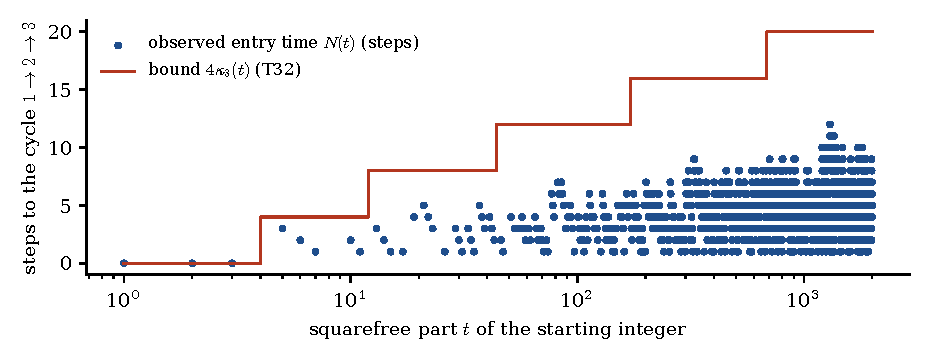
\includegraphics[width=0.9\linewidth]{figs/fig_regimeI.pdf}
\caption{Entry time into the cycle \(1\to2\to3\) of regime I for every squarefree \(t\le2000\) (Theorem~\ref{th:F.T32}); the observed maximum is 12 steps, against the bound \(4\kappa_3(t)\le20\).}\label{fig:regimeI}
\end{figure}

\begin{theorem}[Exact reach counting at \(G=1\)]\rec{F.L4}\scope{C}\label{thm:L4}
After entry into regime~I, the cumulative set of moduli is
\[
U=\bigcup_n\Dx(x_n)=\{q2^k:\ q\mid o,\ k\ge0,\ q2^k\ge2\},
\]
and for every integer \(X\ge1\)
\[
U(X)=\#\{d\in U:d\le X\}=\sum_{q\mid o,\ q\le X}\Big(1+\lfloor\log_2(X/q)\rfloor\Big)-1 .
\]
Hence \(U(X)=\tau(o)\log_2X+O(1)\) and \(U\) has natural density zero.
\end{theorem}
\begin{proof}
By monotonicity \(\Dx_n\subseteq\Dx_N\) for \(n\le N\), and \(\Dx_N\) is the set of divisors \(\ge2\) of \(s_N=2^{k_N}o\), contained in the displayed set. For \(n\ge N\), \(s_n=2^{k_n}o\) with \(k_n\to\infty\), and \(\Dx_n\) is the set of divisors \(\ge2\) of \(s_n\). The union is the displayed set. The count is the number of pairs \((q,k)\) with \(q\mid o\), \(q2^k\le X\), minus the pair \((1,0)\).
\end{proof}

\section{Modular escape and the first exclusions}

A fibre cannot stand still for long when \(G>1\): the progression it follows eventually meets the integers divisible by 4, where \(G\) would be 1.

\begin{lemma}[Modular escape]\rec{F.L1}\scope{C}\label{lem:escape}
Let \(G(x)=g>1\) and suppose \(\Dx\) is unchanged for steps \(0,\dots,k\). Put \(y_j=gx_j=y_0+jL^2\). If \(L\) is odd, there is \(k_*\in[1,4g]\) with \(y_{k_*}\equiv0\ (\mathrm{mod}\ 4g)\); if \(L\) is even (then \(g\) is odd), there is \(k_*\in[1,g]\) with the same property. In either case \(\Dx\) cannot be unchanged through step \(k_*\).
\end{lemma}
\begin{proof}
If \(L\) is odd, \(\gcd(L^2,4g)=1\) and \(y_0+jL^2\equiv0\ (\mathrm{mod}\ 4g)\) is solvable with \(1\le j\le4g\). If \(L\) is even, then \(g\) is odd (for even \(g\) every \(d\equiv1\ (\mathrm{mod}\ g)\) is odd), an even \(d\in\Dx\) gives \(4\mid a\), hence \(4\mid y_0=a(g/b)\), and \(y_j=4(y_0/4+j(L/2)^2)\) with \(\gcd((L/2)^2,g)=1\); so \(y_j\equiv0\ (\mathrm{mod}\ 4g)\) iff \(y_0/4+j(L/2)^2\equiv0\ (\mathrm{mod}\ g)\), solvable with \(1\le j\le g\). If \(\Dx\) were unchanged through \(k_*\), then \(x_{k_*}=y_{k_*}/g\) would be an integer divisible by 4, so \(G(x_{k_*})=1\) by Theorem~\ref{thm:G-arith}(c), contradicting \(G(x_{k_*})=g>1\).
\end{proof}

\begin{proposition}[Plateau escape]\rec{F.T37}\scope{C}\label{th:plateau-escape}
In an orbit with \(G=g>1\) at the start of a plateau, the plateau has at most \(4g\) steps if \(L\) is odd and at most \(g\) steps if \(L\) is even. Consequently a persistent orbit (one with \(G_n=g>1\) for all large \(n\)) has infinitely many growth events, all \(G\)-preserving.
\end{proposition}
\begin{proof}
The first assertion is Lemma~\ref{lem:escape}. If \(G_n=g\) for all \(n\ge n_0\), every plateau is finite, so there are infinitely many growth events; none reduces \(G\), by persistence.
\end{proof}

\begin{theorem}[Collapse from \(G=2,3,6\)]\record{F.T34, F.L2}\label{th:F.T34}\label{th:F.L2}\scope{C}\label{thm:G236}
If \(G(x)=2\) then \(G(x_n)=1\) for some \(n\le7\). If \(G(x)=3\) then \(G(x_n)=1\) for some \(n\le2\). If \(G(x)=6\) then \(G(x_n)=1\) for some \(n\le29\). In particular none of \(2,3,6\) is the limit \(G_\infty\) of an orbit.
\end{theorem}
\begin{proof}
\emph{\(G=2\).} All \(d\) are odd, so \(L\) is odd and \(L^2\equiv1\ (\mathrm{mod}\ 8)\). With \(y=2x\), \(y'=y+L^2\), so while \(G=2\) the residue \(y\bmod8\) increases by one per step, even across growth events. Initially \(y\not\equiv0\ (\mathrm{mod}\ 8)\), since otherwise \(x\in4\Z\) and \(G=1\). Within seven steps \(y\equiv0\ (\mathrm{mod}\ 8)\) would occur; at that state \(x\) is an integer divisible by 4, so \(G=1\). Since \(G\) can only decrease through divisors of 2, \(G\) reaches 1 within seven steps.

\emph{\(G=3\).} If all \(d\) were odd, \(2\mid G\); so \(L\) is even and \(4\mid a\), hence \(4\mid y=3x\). While \(G=3\), \(y/4\) increases by \((L/2)^2\equiv1\ (\mathrm{mod}\ 3)\) per step, starting from a nonzero residue (otherwise \(x\in4\Z\)). Within two steps \(y/4\equiv0\ (\mathrm{mod}\ 3)\), i.e. \(x=4(y/4)/3\) is an integer divisible by 4 and \(G=1\).

\emph{\(G=6\).} Every \(d\equiv1\ (\mathrm{mod}\ 6)\) is coprime to 6, so \(L^2\equiv1\ (\mathrm{mod}\ 24)\), and \(y=6x\) increases by one modulo 24 per step while \(G=6\), starting nonzero. At the step \(k^*\le23\) with \(y\equiv0\ (\mathrm{mod}\ 24)\) the value \(x\) is an integer divisible by 4, so \(G=1\) there at the latest. If \(G\) first drops to 2 or 3, this happens at a step \(j\le22\), after which at most 7 further steps are needed; so \(G=1\) within \(22+7=29\) steps.
\end{proof}

\begin{figure}[t]
\centering
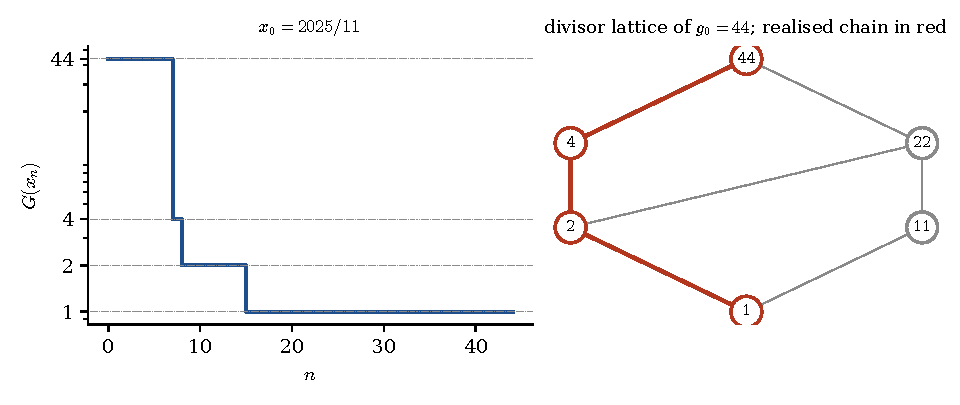
\includegraphics[width=0.97\linewidth]{figs/fig_gchain.pdf}
\caption{A divisor chain of \(G\) in an actual orbit. Left: \(G(x_n)\) for \(x_0=2025/11\) steps down \(44\to4\to2\to1\). Right: the divisor lattice of \(g_0=44\) with the realised chain in red. Each step of the chain is a reducing event, so \(G_{n+1}\mid G_n\) (Theorem~\ref{thm:mono}); the values \(2\) and \(4\) are transient by Theorems~\ref{thm:G236} and~\ref{thm:G24}.}\label{fig:gchain}
\end{figure}


Theorem~\ref{thm:G236} removes three values; Theorem~\ref{thm:G24} of the next chapter removes every divisor of 24 and Theorem~\ref{thm:Pg} shows that these are not the only obstructions that can occur.

\section{Transitions between fibres}

How does a new modulus enter the fibre? The following criterion gives the exact answer in terms of \(y=Gx\).

\begin{theorem}[Transition criterion]\rec{F.T35}\scope{C}\label{thm:transition}
Let \(x\) be realised, \(g=G(x)\), \(L=L(x)\), \(y=gx\), \(Y=y+L^2\), so that \(C(x)=Y/g\). For every integer \(d\ge2\),
\[
d\in\Dx(C(x))\iff d^2\mid Y\ \text{ and }\ \frac{g}{\gcd(g,d-1)}\ \Big|\ \frac{Y}{d^2}.
\]
Consequently \(G(C(x))=\gcd\big(g,\{d-1:d\in\Dx(C(x))\setminus\Dx(x)\}\big)\) (the gcd with the empty set is \(g\)). A step is therefore of exactly one of three kinds: \emph{none} (\(\Dx'=\Dx\)); \emph{preserving} (\(\Dx'\supsetneq\Dx\), every new \(d\equiv1\ (\mathrm{mod}\ g)\), \(G'=g\)); \emph{reducing} (some new \(d\not\equiv1\ (\mathrm{mod}\ g)\), \(G'<g\)). A modulus \(d\equiv1\ (\mathrm{mod}\ g)\) lies in \(\Dx(C(x))\) iff \(d^2\mid Y\).
\end{theorem}
\begin{proof}
By Volume~I (Theorem~1.2), \(d\in\Dx(x')\) iff \(x'(d-1)/d^2\) is a positive integer, i.e. \(Y(d-1)/(gd^2)\in\Z_{>0}\). As \(\gcd(d^2,d-1)=1\), this forces \(d^2\mid Y\), and then it reads \(g\mid(Y/d^2)(d-1)\), i.e. \(g/\gcd(g,d-1)\mid Y/d^2\). The converse is the same chain. The formula for \(G'\) follows from \(\Dx\subseteq\Dx'\): \(G'=\gcd(G,\gcd\{d-1:d\in\Dx'\setminus\Dx\})\). If \(d\equiv1\ (\mathrm{mod}\ g)\), then \(\gcd(g,d-1)=g\) and the second condition is vacuous.
\end{proof}

\begin{theorem}[Anatomy of a preserving event]\rec{F.T36}\scope{C}\label{thm:anatomy}
Let \(x\to x'\) be a preserving event, \(g=G(x)\), \(y=gx\), \(Y=y+L^2\), and \(\mathcal N=\Dx(x')\setminus\Dx(x)\). Then:
\begin{enumerate}[label=(\alph*),nosep]
\item every \(d\in\mathcal N\) is coprime to \(g\);
\item no \(d\in\mathcal N\) divides \(L\); thus each \(d\in\mathcal N\) contains a \emph{fresh prime} (\(q\nmid L\)) or a \emph{carried prime power} (\(\vv_q(d)>\vv_q(L)>0\));
\item for a fresh prime \(q\mid d\): \(q\nmid y\), \(q\nmid g\), and \(y\equiv-L^2\ (\mathrm{mod}\ q^2)\), i.e. \(-y\) is a nonzero square modulo \(q^2\);
\item for a carried prime \(q\), \(l=\vv_q(L)\): \(\vv_q(y)=2l\) exactly, and \(q\mid y/q^{2l}+(L/q^l)^2\);
\item \(\mathcal N\) is closed under divisors in the residue class: if \(d\in\mathcal N\), \(e\mid d\), \(e\ge2\), \(e\equiv1\ (\mathrm{mod}\ g)\), then \(e\in\mathcal N\cup\Dx(x)\).
\end{enumerate}
\end{theorem}
\begin{proof}
(a) \(d\equiv1\ (\mathrm{mod}\ g)\). (b) If \(d\mid L\) and \(d\equiv1\ (\mathrm{mod}\ g)\), then \(d^2\mid L^2\mid y=a(g/b)\) and \(\gcd(d,g)=1\) give \(d^2\mid a\); also \(d\equiv1\ (\mathrm{mod}\ b)\) since \(b\mid g\); so \(d\in\Dx(x)\), contradicting newness. Hence some prime \(q\) has \(\vv_q(d)>\vv_q(L)\), which is the fresh or carried case. (c) \(d^2\mid Y\) (Theorem~\ref{thm:transition}) gives \(q^2\mid y+L^2\); \(q\nmid L\) then forces \(q\nmid y\), and \(q\nmid g\) by (a). (d) \(\vv_q(Y)\ge2\vv_q(d)>2l\) while \(\vv_q(L^2)=2l\) and \(\vv_q(y)\ge2l\) (Proposition~\ref{prop:frame}(c)); the valuation of the sum exceeds \(2l\) only if \(\vv_q(y)=2l\) and the \(q\)-free parts cancel modulo \(q\). (e) \(e^2\mid d^2\mid Y\) and \(e\equiv1\ (\mathrm{mod}\ g)\); Theorem~\ref{thm:transition} gives \(e\in\Dx(x')=\Dx\cup\mathcal N\).
\end{proof}

\emph{Reading.} A preserving event is never an internal rearrangement of the present fibre. It introduces either a new prime, through an arithmetic coincidence \(y\equiv-L^2\ (\mathrm{mod}\ q^2)\), or raises the exponent of a prime already present, a \emph{carry}. Carries are the events that drive the whole theory of Chapters~\ref{ch:gamma}--\ref{ch:bounds}.

\section{The reach set and non-universality}

The union \(U=\bigcup_n\Dx(x_n)\) is infinite (Theorem~\ref{thm:growth}). It is nevertheless sparse.

\begin{theorem}[Non-universality of reach]\rec{F.T33}\scope{C}\label{thm:nonuniv}
Let \(G_\infty=\lim G_n\) (the limit exists: \(G_{n+1}\mid G_n\)).
\begin{enumerate}[label=(\Alph*),nosep]
\item If \(G_\infty>1\), then \(U\subseteq\{d\ge2:d\equiv1\ (\mathrm{mod}\ G_\infty)\}\); in particular \(2\notin U\), \(U\) contains no multiple of \(G_\infty\), and \(U\) has upper asymptotic density at most \(1/G_\infty\).
\item If \(G_\infty=1\), the orbit is eventually in regime~I and \(U=\{q2^k:q\mid o,\,k\ge0\}\setminus\{1\}\) is exactly as in Theorem~\ref{thm:L4}; every \(d\) having an odd prime factor outside \(o\) is never reached, and \(U(X)=O(\log X)\).
\end{enumerate}
Hence for every orbit the reach set \(U\) omits infinitely many integers \(d\ge2\): not every index is ever reached, although the fibre grows without bound.
\end{theorem}
\begin{proof}
For every \(n\), each \(d\in\Dx_n\) satisfies \(d\equiv1\ (\mathrm{mod}\ G_n)\), hence modulo \(G_\infty\mid G_n\). This gives (A). In case (B), \(G_{n_0}=1\) for some \(n_0\), so \(x_{n_0}\) is an integer divisible by 4 (Theorem~\ref{thm:G-arith}), regime~I applies (Theorem~\ref{thm:regimeI}), and Theorem~\ref{thm:L4} gives \(U\); moduli at earlier steps lie in \(\Dx_{n_0}\) by monotonicity. For the counting: \(U(X)\le\tau(o)(1+\log_2X)\).
\end{proof}

For instance the orbit of \(4\) is \(4,8,12,16,32,48,64,128,\dots\) and reaches only powers of two.

\begin{remark}[Scope of the density statement]\rec{F.L5}\scope{C}\label{rem:L5}
Part (A) proves, for \(G_\infty>1\), the upper density bound \(1/G_\infty\) and the exclusion of infinitely many moduli. The logarithmic counting function and density zero are proved above for \(G_\infty=1\). That they hold for \emph{every} orbit, including those with \(G_\infty>1\), is a consequence of single-prime dominance and is proved in Corollary~\ref{cor:logreach}. In this form non-universality is established for all collective orbits and the density statement is stated exactly where it is proved.
\end{remark}
